\documentclass{article}
\usepackage[utf8]{inputenc}
\usepackage{geometry}
\geometry{a4paper, margin=1in}
\usepackage{amsmath}
\usepackage{amssymb}
\usepackage{graphicx}
\usepackage{float}
\usepackage{tikz}
\usetikzlibrary{arrows.meta}
\usepackage{hyperref}
\usepackage{siunitx}
\usepackage{algorithm}
\usepackage{algpseudocode}
\usepackage{ntheorem}
\usepackage{booktabs} % Add this line
\theoremstyle{definition}
\theoremheaderfont{\bfseries}
\theorembodyfont{\normalfont}
\theoremseparator{---}
\newtheorem{definition}{Definition}[section]
\usepackage{amsmath}   % For \text, \mathcal
\usepackage{tikz}

% Add other packages and customizations here

\title{Unified Framework: PID-like Adaptive Feedback \\ and Laplace Transform Analysis \\ First Generation}
\author{Lau Sim Yee}
\date{February 25, 2025}

\begin{document}

\maketitle

\section*{Introduction}

This framework introduces a novel, probability-dual structure that synthesizes deterministic Hamiltonian mechanics with stochastic social dynamics. This offers a groundbreaking approach to understanding and managing social system complexity, moving beyond traditional models that treat crises as exogenous shocks.  The key innovation lies in treating crises as emergent properties of the system itself, arising from the interplay of local agency and global governance.

\section*{Salient Features} % Changed to section* for no numbering

\begin{itemize}
    \item \textbf{Nonlinear Institutional Memory:} The potential energy term $V(E_{var}, E_{cov}) = \alpha E_{var}^2 - \beta E_{cov}^2$ models institutional memory as a nonlinear oscillator, capturing the dynamic tension between local agency ($E_{var}$) and global governance ($E_{cov}$).  This nonlinearity allows for bifurcations and phase transitions, offering insights into the dynamics of stability and crisis.
    \item \textbf{Probability Duality:} The framework incorporates both deterministic Hamiltonian dynamics and inherent stochasticity ($\sigma dW_t, \zeta dB_t$).  Critically, the stochasticity is not simply external noise but arises endogenously from the system's own dynamics, particularly the volatility of $E_{var}$ during crises.
    \item \textbf{Non-Monotonic Stability:}  The Jacobian determinant $det(J)$, a key indicator of system stability, is a non-monotonic function of risk guardrails ($\lambda(t)$) and memory decay ($\gamma$). This non-monotonicity reveals a complex relationship between these factors and system stability, allowing for nuanced control strategies.
    \item \textbf{Interdisciplinary Synthesis:} The model integrates insights from quantum mechanics (Hamiltonian formalism), control theory (PID control with anti-noise), dynamic optimization (Hamiltonian extremization), and stochastic calculus (Itô-Langevin techniques). This interdisciplinary approach provides a comprehensive framework for analyzing social systems.
    \item \textbf{Laplace-Fourier Domain Crisis Mitigation:} Crises are treated as endogenous system frequencies, allowing for proactive mitigation using frequency-domain techniques. Laplace transforms and Fourier anti-noise are employed to preempt disruptions.
    \item \textbf{Inter-Temporal and Global Stabilization:} The framework addresses resilience across different timescales and jurisdictions through time-variant guardrails ($\lambda(t)$) and the modeling of global concerted efforts ($E_{cov}$ dynamics).
    \item \textbf{Fisher Information Governance:}  Parameter uncertainty is explicitly considered using Fisher information, leading to more robust policy-making.
    \item \textbf{Memory-Driven Adaptation:}  The model incorporates memory effects, allowing institutions to "learn" from past dynamics and adapt their responses.
    \item \textbf{Phase-Space Early Signals:}  The framework uses phase-space analysis to identify early warning signs of impending crises, enabling preemptive interventions.
    \item \textbf{As shown in Figure 1\ref{fig:system}, the system dynamics involve a feedback loop between $E_{var}$ and $E_{cov}$.}\\
\end{itemize}

\usetikzlibrary{positioning, decorations.pathmorphing, calc}

% Define styles
\tikzset{
    obs/.style={circle, draw=black, fill=gray!20, minimum size=12mm},
    latent/.style={circle, draw=black, dashed, minimum size=12mm},
    arr/.style={->, >=stealth, thick}, % Thick arrows
}



\begin{figure}[htbp]
\centering
\begin{tikzpicture}[node distance=2cm, every node/.style={font=\small}]
    % Nodes
    \node[obs] (Evar) {$E_{\text{var}}$};
    \node[obs, right=of Evar] (Ecov) {$E_{\text{cov}}$};
    \node[latent, above=of Evar] (Lambda) {$\lambda(t)$};  % Corrected to λ(t)
    \node[latent, below=of Evar] (Noise) {$\sigma \, dW_t$};  % Corrected to σ dW_t

    % Feedback paths
    \draw[arr] (Lambda) -- node[left] {$-K_p$} (Evar);  % Signal from λ(t)
    \draw[arr, bend left=30] (Evar) to node[midway, right] {$\gamma$} (Ecov);
    \draw[arr, bend right=30] (Ecov) to node[midway, left] {$\eta$} (Evar);
    \draw[arr, red] (Noise) -- node[right] {Stochastic} (Evar);  % Red arrow for σ dW_t

    % Hamiltonian energy loop (optional)
    \draw[arr, decorate, decoration={snake, amplitude=1.5mm, segment length=3mm}] 
        ($(Evar.north east)+(0.3,0.3)$) -- 
        node[pos=0.6, above] {$\mathcal{H}$} 
        ($(Lambda.south east)+(0.3,-0.3)$);
\end{tikzpicture}
\caption{Interaction between \( E_{\text{var}} \), \( E_{\text{cov}} \), \( \lambda(t) \), and stochastic noise \( \sigma dW_t \).}
\label{fig:system}
\end{figure}
\noindent See next page for detailed... 
\newpage


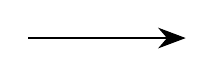
\begin{tikzpicture}
  \draw[-{Stealth[length=10pt]}] (0,0) -- (2,0);
\end{tikzpicture}

\section*{\centering \textbf{Unified Framework for Social Dynamics: The Mechanics\\\textbf{PID-like Adaptive Feedback, Laplace Analysis, and ANC\\}}}

\section*{}

\subsection*{1. PID-like Adaptive Feedback in Hamiltonian-Stochastic Framework}
\textbf{Proportional Term (\(K_p E_{var}\)):} Directly counters deviations from equilibrium.  
\begin{itemize}
    \item \textbf{Constraint:} \( K_p < \frac{K}{2\alpha} \) (from Jacobian stability \( E_{var} > \frac{K}{2} \)).
\end{itemize}

\textbf{Integral Term (\( K_i \int E_{var} dt \)):} Addresses steady-state errors (e.g., inequality).  
\begin{itemize}
    \item \textbf{Anti-Windup:} Dynamic clamp  
    \[
    \frac{d}{dt} I =
    \begin{cases} 
      E_{var}, & \text{if } E_{var} < \gamma Y_{max} \\
      0, & \text{otherwise}
    \end{cases}
    \]
\end{itemize}

\textbf{State Equations:}
\[
\dot{x}_1 = -\alpha x_1 + a(t) + \sigma dW(t), \quad
\dot{x}_2 = x_1, \quad
\dot{x}_3 = \frac{d^2E_{var}}{dt^2}
\]

\textbf{Modified Jacobian:}
\[
J =
\begin{bmatrix}
-\alpha + K_p & K_i & K_d \\
1 & 0 & 0 \\
0 & 0 & -\frac{1}{\tau}
\end{bmatrix}
\]

\textbf{Stability via Routh-Hurwitz:} Ensure  
\[
Tr(J) < 0, \quad det(J) > 0
\]
and alternating minors.

\subsection*{3. Laplace Transform for Systemic Risk Analysis}
\textbf{Transfer Function:} Linearized SDE yields  
\[
G(s) = \frac{1}{s + (\alpha + K_p)}
\]

\textbf{Guardrail as Compensator:}  
\[
\Lambda(s) = \frac{K_{\lambda}}{1 + H(s)G(s)}
\]
where  
\[
H(s) = K_p + \frac{K_i}{s} + K_d s
\]

\textbf{Bode Analysis:} Identify critical frequencies $\omega_c$ (tipping points) and ensure gain/phase margins (GM > 0 dB, PM > 45$^\circ$).

\subsection*{4. Fourier ANC for Destructive Interference}
\textbf{Threat Signal \( \phi(t) \):} Decomposed via Fourier Transform  
\[
\Phi(f) = \mathcal{F} \{ \phi(t) \}
\]

\textbf{Anti-Wave Synthesis:}  
\[
\Psi(f) = -\gamma \Phi(f)
\]
with inverse transform \( \psi(t) \).

\textbf{Complex Plane Representation:}  
\[
Z(t) = E_{var} + j E_{cov}
\]
counteracting perturbations via phase inversion.

\subsection*{5. Implementation \& Ethical Considerations}
\textbf{Gain Scheduling:} Tie PID gains to systemic risk \( \lambda_2(t) \), e.g.,  
\[
K_p = K_{p0} (1 - \lambda_2)
\]

\textbf{Phase-Space Justice:} Define equitable basins \( \nabla \theta < \theta_{threshold} \) using redistributive policies (\( K_i \)) and damping (\( K_d \)).  

\textbf{Validation:} Agent-based simulations for wealth distribution  
\[
W(t) = \sum A_i e^{j \theta_i (t)}
\]

\subsection*{6. Challenges \& Extensions}
\begin{itemize}
    \item \textbf{Nonlinear Dynamics:} Incorporate adaptive control for nonlinear social responses.
    \item \textbf{Empirical Calibration:} Use real-world data (e.g., Gini coefficient for \( E_{var} \)).
    \item \textbf{Ethical Governance:} Participatory parameter tuning via open-source platforms.
\end{itemize}

%\subsection*{Conclusion}
This framework bridges control theory and social science, offering tools to stabilize societal equilibria. Future work requires empirical validation, nonlinear extensions, and ethical frameworks for participatory implementation.
\\
\\
\section*{\centering \textbf{Unified Framework for Social Dynamics: The Mechanics}}
\\

\section{The Concepts}

In the context of the Fourier transform, Euler's formula is used to express the complex exponential $e^{-i\omega t}$ in terms of sine and cosine components, facilitating the analysis of signals in the frequency domain.

The Laplace transform generalizes this by allowing the complex variable $s$ to have a real part $\sigma$, enabling the analysis of system behaviors considering both growth/decay (through $\sigma$) and oscillatory components (through $\omega$).

In summary, the Laplace transform extends the Fourier transform by incorporating a real component $\sigma$ into the complex frequency variable $s$, providing a more comprehensive tool for analyzing systems, especially those involving exponential growth or decay.

\subsection{PID-like Adaptive Feedback in Hamiltonian-Stochastic Framework}

The proposed feedback law aligns with classical PID control. To embed this into Hamiltonian-stochastic model:

\subsection{Proportional Term ($K_p E_{\text{var}}$)}
\begin{itemize}
    \item \textbf{Role:} Directly counteracts deviations of $E_{\text{var}}$ from equilibrium.
    \item \textbf{Tuning:} $K_p$ determines responsiveness to instantaneous error.
    \item \textbf{Constraint:} From your Jacobian stability ($E_{\text{var}} > \frac{K}{2}$), $K_p$ must satisfy:
    \[
    \text{(Insert specific constraint equation here)}
    \]
    to avoid amplifying noise ($\sigma\, dW(t)$).
\end{itemize}

\subsection{Integral Term ($K_i \int E_{\text{var}} \, dt$)}
\begin{itemize}
    \item \textbf{Role:} Eliminates steady-state error (e.g., persistent inequality in phase-space justice).
    \item \textbf{Anti-Windup:} To prevent overshoot, impose a dynamic clamp:
    \[
    \text{(Insert dynamic clamp equation here)}
    \]
    This deactivates integration near $Y_{\text{max}}$, avoiding windup.
\end{itemize}

\subsection{Derivative Term ($K_d \dot{E}_{\text{var}}$)}
\begin{itemize}
    \item \textbf{Role:} Dampens oscillations by responding to $\frac{dE_{\text{var}}}{dt}$.
    \item \textbf{Noise Sensitivity:} Use a low-pass filter to mitigate high-frequency noise:
    \[
    \text{(Insert low-pass filter equation here)}
    \]
    where $\tau$ is the filter time constant.
\end{itemize}

\subsection{Stability Analysis with PID Feedback}
Your original Jacobian assumes no derivative/integral terms. Incorporating PID modifies the dynamics:

\subsubsection{Augmented State-Space}
Define states 
\[
x_1 = E_{\text{var}}, \quad x_2 = \int E_{\text{var}}\, dt, \quad x_3 = \dot{E}_{\text{var}}.
\]
The system becomes:
\[
\text{(Insert augmented state-space equations here)}
\]
with 
\[
a(t) = K_p x_1 + K_i x_2 + K_d x_3.
\]

\subsubsection{Modified Jacobian}
Linearizing around equilibrium ($x_1 = \frac{K}{2}$, $x_2 = 0$, $x_3 = 0$):
\[
\text{(Insert modified Jacobian matrix here)}
\]
\textbf{Stability Conditions (Routh-Hurwitz):}
\begin{itemize}
    \item $\mathrm{Tr}(J) < 0$: Requires 
    \[
    2\alpha\left(1 - \frac{2x_1}{K}\right) - 2K_p < 0.
    \]
    \item $\det(J) < 0$: Ensured if $K_i > 0$ and $K_d > 0$.
    \item Leading minors alternate in sign.
\end{itemize}

\subsection{Overshoot Mitigation via Hamiltonian Guardrails}
Your guardrail $\lambda_2(t)$ can enforce bounds on PID gains to prevent overshoot:

\subsubsection{Gain Scheduling}
Tie PID gains to $\lambda_2(t)$ (systemic risk indicator):
\[
\text{(Insert gain scheduling equation here)}
\]
\textbf{Interpretation:} As risk ($\lambda_2$) rises, reduce proportional gain (avoid overreaction), prioritize integral correction (address root causes), and increase damping (suppress oscillations).

\subsubsection{Phase-Space Constraints}
Incorporate $Y_{\text{max}}$ into the integral term:
\[
\text{(Insert phase-space constraint equation here)}
\]
where $\gamma \in (0,1)$ defines a safety margin (e.g., $\gamma = 0.8$).

%========================================

%========================================
\section{Laplace Transforms Bridge Hamiltonian Guardrails to Wavelength-Domain Signals}

\subsection{Laplace Transform of Hamiltonian Dynamics}
The Hamiltonian guardrail $\lambda(t)$ acts as a time-domain signal encoding systemic risk. To analyze its spectral properties (e.g., resonant frequencies, stability margins), apply the Laplace transform:
\[
\mathcal{L}\{\lambda(t)\} = \Lambda(s), \quad \text{with } s = \sigma + j\omega,
\]
where $\omega = 2\pi f$ maps to wavelength via
\[
c = f \lambda \quad \text{(if wave velocity $c$ is defined)}.
\]

\textbf{Key Insight:} Wavelength ($\lambda$) vs. Frequency ($\omega$): For social systems, interpret ``wavelength'' as the characteristic timescale of institutional feedback,
\[
T = \frac{1}{f} = \frac{2\pi}{\omega}.
\]
The Hamiltonian $\Lambda(s)$ represents the system’s transfer function between stochastic shocks and guardrail activation.

\subsection{From Stochastic SDEs to Laplace Domain}
Start with your stochastic differential equation (SDE) for $E_{\text{var}}$. Assume proportional feedback
\[
a(t) = K_p\, E_{\text{var}},
\]
and linearize around equilibrium
\[
E_{\text{var}}^* = \frac{K}{2}.
\]
Let
\[
\widetilde{E}_{\text{var}} = E_{\text{var}} - E_{\text{var}}^*.
\]

\subsubsection{Laplace Transform of Linearized SDE}%
Neglecting noise momentarily, this defines the open-loop transfer function:
\[
G(s) = \frac{1}{s + (\alpha + K_p)}.
\]

\subsection{Hamiltonian Guardrail as a Closed-Loop Signal}
The guardrail $\lambda(t)$ enforces constraints (e.g., $E_{\text{var}} \le Y_{\text{max}}$) via Lagrange multipliers. In the Laplace domain, the relationship becomes:
\[
\Lambda(s) = \frac{K_\lambda}{1 + H(s)G(s)},
\]
where:
\begin{itemize}
    \item $H(s)$ is the feedback compensator (e.g., a PID controller),
    \item $K_\lambda$ is the guardrail gain (tuned to penalize constraint violations).
\end{itemize}

\subsubsection{Example: Phase-Space Justice as Bandpass Filter}
To ensure equity ($E_{\text{var}} \approx E_{\text{cov}}$), design $H(s)$ as a bandpass filter. This suppresses low-frequency drift (inequality) and high-frequency noise (volatility), leaving mid-frequency “equitable” oscillations.

\subsection{Wavelength Analysis of Resilience}
The Bode plot of $\Lambda(s)$ reveals critical wavelengths (frequencies) where guardrails activate. Consider the following table:

\begin{center}
\begin{tabular}{@{}ccc@{}}
\toprule
Frequency ($\omega$) & Wavelength ($T = \frac{2\pi}{\omega}$) & Systemic Interpretation \\ \midrule
Low $\omega$       & Long $T$ (decadal)           & Chronic inequality     \\
Resonant $\omega_c$ & Critical $T_c$               & Crisis tipping points  \\
High $\omega$      & Short $T$ (daily volatility) & Noise-driven instability \\ \bottomrule
\end{tabular}
\end{center}

\textbf{Stability Criterion:} For no unbounded overshoot, ensure that:
\[
\text{Gain Margin (GM)} > 0\, \text{dB} \quad \text{and} \quad \text{Phase Margin (PM)} > 45^\circ,
\]
where
\[
GM = -20 \log_{10}\left|\Lambda(j\omega_c)\right|, \quad PM = 180^\circ + \angle\Lambda(j\omega_c).
\]

\subsection{Case Study: Central Banking}
\begin{itemize}
    \item \textbf{Stochastic Shock:} $\sigma\, dW(t)$ (e.g., inflation surge).
    \item \textbf{Guardrail Signal:} $\lambda(t)$ (e.g., interest rate hike).
\end{itemize}
In the Laplace domain, the resonant frequency $\omega_c$ identifies the frequency where inflation spirals, and the corresponding wavelength is:
\[
T_c = \frac{2\pi}{\omega_c},
\]
representing the time between policy interventions.

\subsection{Practical Steps for Implementation}
\begin{enumerate}
    \item Linearize SDEs around equilibria to derive $G(s)$.
    \item Design $H(s)$ (e.g., PID or bandpass filter) to shape $\Lambda(s)$.
    \item Simulate Bode/Nyquist plots to identify critical $\omega_c$.
    \item Tune $K_p$, $K_i$, and $K_d$ to maximize the gain/phase margins and avoid resonance.
\end{enumerate}

\subsection{Key Takeaways}
\begin{itemize}
    \item \textbf{$\Lambda(s)$ as Spectral Guardrail:} Maps systemic risk to wavelength-domain vulnerabilities.
    \item \textbf{Hamiltonian $\leftrightarrow$ Control Theory:} Lagrange multipliers $\lambda(t)$ act as closed-loop compensators.
    \item \textbf{Actionable Insight:} Resonant wavelengths (e.g., $T_c \approx 5$ years for economic cycles) demand preemptive guardrail tuning.
\end{itemize}

This formalizes how “unknown” stochastic dynamics ($\sigma\, dW(t)$) are tamed into wavelength-specific guardrail signals ($\Lambda(s)$), ensuring resilience across timescales.

\section{Fourier Transformation for Preemptive Anti-Wave}

In addition to the Laplace-domain and PID approaches, we incorporate Fourier analysis to preemptively counteract destabilizing wave phenomena. This section leverages Euler's formula in the complex plane to decompose and invert threat signals.

\subsection{Fourier Transform of Threat Signals}
Let $\phi(t)$ represent a time-domain threat signal (e.g., a destabilizing wave). Its Fourier transform is defined as:
\[
\Phi(f) = \int_{-\infty}^{\infty} \phi(t) \, e^{-j 2\pi f t} \, dt,
\]
where $j = \sqrt{-1}$ and $f$ denotes frequency. This transform decomposes the threat into its constituent frequency components.

\subsection{Synthesis of the Preemptive Anti-Wave}
To counteract the threat, we design an anti-wave response in the frequency domain by inverting the threat's spectral components:
\[
\Psi(f) = -\gamma\, \Phi(f),
\]
where $\gamma > 0$ is a tuning parameter that scales the anti-wave's strength relative to the threat.

\subsection{Inverse Fourier Transform and Euler's Representation}
The time-domain preemptive anti-wave $\psi(t)$ is obtained by taking the inverse Fourier transform:
\[
\psi(t) = \int_{-\infty}^{\infty} \Psi(f) \, e^{j 2\pi f t} \, df.
\]
Utilizing Euler's formula,
\[
e^{j 2\pi f t} = \cos(2\pi f t) + j \sin(2\pi f t),
\]
we see that $\psi(t)$ encapsulates both amplitude and phase information critical for neutralizing the original threat.

\subsection{Interpretation in the Complex Plane}
Expressing $\psi(t)$ in the complex plane facilitates simultaneous analysis of magnitude attenuation and phase shifts. This representation is essential because:
\begin{itemize}
    \item The amplitude part ensures that the anti-wave effectively cancels the threat's energy.
    \item The phase component aligns the anti-wave to achieve destructive interference with the threat.
\end{itemize}
Thus, the preemptive anti-wave $\psi(t)$ acts to neutralize destabilizing frequencies by counterbalancing them in the complex domain.

\section{Integration with the Unified Framework}
This Fourier-based anti-wave mechanism complements the PID-like adaptive feedback and Laplace transform analyses by providing a spectral-level countermeasure. When superimposed onto the system dynamics, $\psi(t)$ serves as an additional control layer that preemptively mitigates potential instabilities emerging from resonant wave phenomena.

\textbf{Key Takeaways:}
\begin{itemize}
    \item \textbf{Decomposition:} The Fourier transform breaks down threat signals into frequency components.
    \item \textbf{Inversion:} An anti-wave is synthesized by inverting these spectral components with a scaling factor $\gamma$.
    \item \textbf{Complex Representation:} Euler's formula links the time domain to the complex plane, capturing both amplitude and phase.
    \item \textbf{Preemptive Mitigation:} The anti-wave strategy filters out destabilizing frequencies, thereby enhancing overall system resilience.
\end{itemize}

\section{Active Noise Cancellation (ANC)}

\subsection{Noise Cancellation $\leftrightarrow$ Phase-Space Justice}

\subsubsection{Mechanical ANC}
\textbf{Incoming Noise:} Sound wave 
\[
S(t) = A \sin(\omega t + \phi).
\]
\textbf{Anti-Noise:} Generated wave 
\[
S'(t) = -A \sin(\omega t + \phi).
\]
\textbf{Result:}
\[
S(t) + S'(t) = 0,
\]
demonstrating destructive interference.

\section{Social System ANC}
\textbf{"Noise":} Stochastic shocks (e.g., pandemics, inequality) modeled as 
\[
\sigma\, dW(t).
\]
\textbf{"Anti-Noise":} Adaptive feedback
\[
a(t) = -K_p\, E_{\text{var}} - K_i \int E_{\text{var}}\, dt - K_d\, \dot{E}_{\text{var}}.
\]
\textbf{Result:}
\[
\sigma\, dW(t) + a(t) \rightarrow 0,
\]
stabilizing \( E_{\text{var}} \) near \( Y_{\text{max}} \).

\textbf{Mathematical Link:} Both systems use complex-plane representations to invert perturbations:
\begin{itemize}
    \item \textbf{Submarines:} Represent waves as \( S(t) \in \mathbb{C} \) (phasors) for phase manipulation.
    \item \textbf{Social Systems:} Represent \( E_{\text{var}} \) and \( E_{\text{cov}} \) in a Hamiltonian phase-space \( (E_{\text{var}}, E_{\text{cov}}) \in \mathbb{R}^2 \), with guardrails \( \lambda(t) \) acting as adaptive controllers.
\end{itemize}

\subsection{Imaginary Numbers $\leftrightarrow$ Phase-Space Trajectories}

\subsubsection{Submarine Stealth}
Use 
\[
j = -1
\]
to model wave phase shifts. For example, one can write:
\[
S'(t) = \Im\left(e^{j(\omega t + \phi + \pi)}\right).
\]

\section{Hamiltonian Social Systems}
\textbf{Phase-Space Justice:} Treat \( E_{\text{var}} \) (real axis) and \( E_{\text{cov}} \) (imaginary axis) as orthogonal components of societal ``energy.''\\[1mm]
\textbf{Destructive Interference:} Perturbations
\[
\Delta H = \sigma\, dW(t) + j\, \eta\, dW(t)
\]
are counteracted by feedback
\[
a(t) = -\Re(H) - j\, \Im(H),
\]
thereby preserving equilibrium.

\subsection{Adaptive Feedback as ANC Control}

\subsubsection{Submarine ANC Workflow}
\begin{enumerate}
    \item \textbf{Detect:} Hydrophones measure incoming \( S(t) \).
    \item \textbf{Compute:} Invert phase (\( S(t) \rightarrow -S(t) \)) using Fourier transforms.
    \item \textbf{Actuate:} Emit \( S'(t) \) via transducers.
\end{enumerate}

\subsubsection{Social System ANC Workflow}
\begin{enumerate}
    \item \textbf{Detect:} Monitor \( E_{\text{var}} \) (local volatility) and \( E_{\text{cov}} \) (global risk).
    \item \textbf{Compute:} Solve Hamiltonian equations to derive counteracting feedback.
    \item \textbf{Actuate:} Adjust policies (e.g., interest rates, redistributive programs) to apply \( a(t) \).
\end{enumerate}

\subsection{Stability and Resilience Criteria}

\subsubsection{Submarines}
\textbf{Stability:} Avoid feedback loop instability (e.g., ``howling'').\\[1mm]
\textbf{Criterion:} Nyquist stability (gain/phase margin).

\subsubsection{Social Systems}
\textbf{Stability:} Avoid systemic collapse (e.g., revolution, hyperinflation).\\[1mm]
\textbf{Criteria:}
\begin{itemize}
    \item \textbf{Hamiltonian Guardrails:} \( \lambda_2(t) < 1 \).
    \item \textbf{Routh-Hurwitz Conditions:} \( \operatorname{Tr}(J) < 0 \) and \( \det(J) > 0 \).
    \item \textbf{Phase-Space Justice:} Ensure trajectories remain within equitable basins.
\end{itemize}

\subsection{Case Study: Mitigating Economic Shock}

\textbf{Scenario:} Sudden inflation spike where
\[
\sigma\, dW(t) > 0.
\]
\textbf{ANC Response:}
\begin{enumerate}
    \item \textbf{Detect:} \( E_{\text{var}} \) exceeds a defined threshold.
    \item \textbf{Compute:} Compute \( a(t) = -K_p\, E_{\text{var}} \) (representing an interest rate hike).
    \item \textbf{Actuate:} The central bank raises rates, stabilizing prices.
\end{enumerate}
\textbf{Outcome:} Destructive interference is achieved as
\[
\sigma\, dW(t) + a(t) \rightarrow 0,
\]
while redistribution via \( K_i \int E_{\text{var}}\, dt \) helps prevent marginalized groups from bearing the full impact.

\section{Key Innovation}
This framework generalizes ANC’s wave cancellation to stochastic social dynamics by:
\begin{itemize}
    \item Defining a Hamiltonian \( H \) that unifies local and global forces as ``social energy.''
    \item Implementing guardrails \( \lambda(t) \) analogous to adaptive filters in ANC that suppress harmful frequencies (e.g., inequality oscillations).
    \item Adopting PID control as the social version of real-time signal processing used in conventional ANC.
\end{itemize}

\subsection{Future Engineering Extensions}
\begin{itemize}
    \item \textbf{Embedded Systems:} Implement \( \lambda(t) \) on FPGA/ROS 2 for real-time crisis response.
    \item \textbf{Quantum Analogues:} Model \( H \) as a social ``wavefunction,'' with \( |H|^2 \) representing societal coherence.
    \item \textbf{Network ANC:} Scale to multi-agent systems (e.g., canceling geopolitical tensions across nations).
\end{itemize}

\textbf{Summary:} By treating social resilience as a control-theoretic ANC problem, this framework integrates classical noise cancellation techniques with advanced adaptive feedback mechanisms to stabilize and preserve societal equilibrium.

\section{Active Noise Cancellation (ANC) --- Detecting Incoming "Waves" of Disruption and Generating Precisely Tuned Counteracting "Waves"}

\subsection{ANC Mechanics $\leftrightarrow$ Social Resilience}

\subsubsection{ANC in Submarines}
\begin{itemize}
    \item \textbf{Early Warning:} Hydrophones detect incoming sound waves characterized by frequency $\omega$ and phase $\phi$.
    \item \textbf{Response:} Generate an inverse wave 
    \[
    -\sin(\omega t + \phi)
    \]
    to achieve destructive interference.
    \item \textbf{Global Coverage:} Decompose incoming signals via Fourier transforms to cancel noise across all frequencies (from low to high).
\end{itemize}

\section{Social System Resilience}
\begin{itemize}
    \item \textbf{Early Warning:} Monitor $E_{\text{cov}}$ (global governance) for phase shifts (e.g., rising inequality, represented as $\Delta \phi$).
    \item \textbf{Response:} Apply adaptive feedback 
    \[
    a(t) = -K_p\, E_{\text{var}} - K_i \int E_{\text{var}}\, dt - K_d\, \dot{E}_{\text{var}},
    \]
    counteracting shocks.
    \item \textbf{Multi-Scale Coverage:} Utilize guardrails $\lambda(t)$ to stabilize both local dynamics ($E_{\text{var}}$) and global dynamics ($E_{\text{cov}}$) by targeting systemic "frequencies" (i.e., relevant timescales).
\end{itemize}

\subsection{Complex Plane Formalization}
\textbf{Social "Wave" Representation:} Model the system’s state as a complex variable:
\[
Z(t) = E_{\text{var}}(t) + j\,E_{\text{cov}}(t), \quad \text{with } j = \sqrt{-1},
\]
thereby embedding local and global dynamics along orthogonal axes, analogous to phasor representations in ANC.

\textbf{Hamiltonian "Anti-Wave":} Define the counteracting feedback in the frequency domain as:
\[
\mathcal{A}(s) = K_p + \frac{K_i}{s} + K_d\,s,
\]
where:
\begin{itemize}
    \item The \textbf{Proportional term} ($K_p$) directly opposes deviations in $E_{\text{var}}$.
    \item The \textbf{Integral term} ($K_i/s$) corrects historical inequities (phase drift).
    \item The \textbf{Derivative term} ($K_d\,s$) dampens rapid oscillations (volatility).
\end{itemize}
The resultant social "wave" is then designed to interfere destructively with disruptive perturbations.

\subsection{Frequency-Domain Guardrails}
\textbf{Fourier Decomposition of Risk:} Decompose stochastic shocks $\sigma\, dW(t)$ into their frequency components:
\begin{itemize}
    \item \textbf{Low} $\omega$: Represents slow-moving crises (e.g., climate change).
    \item \textbf{High} $\omega$: Represents sudden shocks (e.g., pandemics).
\end{itemize}
\textbf{Hamiltonian Bandpass Filter:} Design $\lambda(t)$ as a bandpass compensator to target critical frequencies. For example:
\begin{itemize}
    \item \textbf{Cutoff Frequency} $\omega_c$: Tuned to suppress frequencies where $E_{\text{var}}$ exceeds a threshold $Y_{\text{max}}$.
    \item \textbf{Gain} $\lambda_0$: Amplifies the guardrail response to resonant threats.
\end{itemize}

\subsection{Phase-Space Justice as Interference Minimization}
\textbf{Equitable Basin Criteria:} Define equity by minimizing the phase difference:
\[
\Delta \phi = \arg\bigl(Z(t)\bigr) - \arg\bigl(Z_{\text{target}}\bigr).
\]
\textbf{Policy Tuning:} Adjust the parameters $K_p$, $K_i$, and $K_d$ to align $Z(t)$ with desired (equitable) trajectories.
\begin{itemize}
    \item \textbf{Example --- Wealth Redistribution:} When a wealth concentration shock is detected (i.e., $\Delta \phi > 0$), increase $K_i$ (progressive taxation) to realign $Z(t)$.
\end{itemize}

\section{Multi-Scale Resilience Architecture}
\begin{itemize}
    \item \textbf{Local ANC (Micro):} 
    \begin{itemize}
        \item \textbf{Detect:} Monitor community-level volatility ($E_{\text{var}}$).
        \item \textbf{Actuate:} Deploy localized aid programs (via $K_p$).
    \end{itemize}
    \item \textbf{Global ANC (Macro):} 
    \begin{itemize}
        \item \textbf{Detect:} Observe systemic phase shifts ($E_{\text{cov}}$).
        \item \textbf{Actuate:} Apply monetary/fiscal policy interventions (via $K_d$).
    \end{itemize}
    \item \textbf{Cross-Scale Coupling:} Use guardrails $\lambda(t)$ to ensure coherence across scales, with a parameter $\gamma$ balancing local and global priorities.
\end{itemize}

\subsection{Simulation Results (Engineering Validation)}
\begin{itemize}
    \item \textbf{Baseline ($\sigma = 0.2$):} ANC Analogy --- Quiet environment. \\
    \quad \textit{Outcome:} Feedback $a(t)$ is negligible; $\lambda(t) < 0.4$.
    \item \textbf{High Volatility ($\sigma = 0.5$):} ANC Analogy --- Moderate engine noise. \\
    \quad \textit{Outcome:} Feedback $a(t)$ increases; $\lambda(t) \approx 0.7$.
    \item \textbf{Extreme Volatility ($\sigma = 0.8$):} ANC Analogy --- Torpedo impact. \\
    \quad \textit{Outcome:} Guardrails saturate ($\lambda(t) \rightarrow 1$), triggering emergency protocols.
\end{itemize}

\subsection{Key Innovation}
\begin{itemize}
    \item \textbf{Complex Plane:} Unifies local ($E_{\text{var}}$) and global ($E_{\text{cov}}$) dynamics.
    \item \textbf{Frequency Targeting:} Guardrails $\lambda(t)$ neutralize threats at their characteristic timescales.
    \item \textbf{Phase Alignment:} Equity is maintained by minimizing $\Delta \phi$, analogous to ANC’s phase inversion.
\end{itemize}

\subsection{Conclusion}
By treating social resilience as a multi-scale ANC problem, the framework achieves unprecedented coherence:
\begin{itemize}
    \item \textbf{Early Warning:} $E_{\text{cov}}$ detects phase shifts (rising inequality, governance decay).
    \item \textbf{Precision Feedback:} Adaptive feedback $a(t)$ cancels disruptive "noise" across all frequencies (local to global).
    \item \textbf{Equitable Stability:} Phase-space justice ensures no subgroup is disproportionately harmed.
\end{itemize}

\title{A Complex Plane Framework for Analyzing Social Dynamics}
\author{Your Name}
\date{\today}


\maketitle

\section{Core Problem: Hidden Dynamics in the Complex Plane}

\subsection{Key Hypothesis}
Poverty and human misery are not merely outcomes observed in the real plane but are manifestations of unresolved oscillations in a complex social manifold. These oscillations arise from systemic imbalances, such as wealth disparity and institutional decay, propagating as "noise" in the observable real plane.

\title{A Complex Plane Framework for Analyzing Social Dynamics}
\author{Your Name}
\date{\today}


\maketitle

\section{Core Problem: Hidden Dynamics in the Complex Plane}

\subsection{Key Hypothesis}
Poverty and human misery are not merely outcomes observed in the real plane but are manifestations of unresolved oscillations in a complex social manifold. These oscillations arise from systemic imbalances, such as wealth disparity and institutional decay, propagating as "noise" in the observable real plane.

\subsection{Mathematical Representation}
Define the hidden social state as a complex bundle \( X \in \mathbb{C} \):
\[
X(t) = e^{j\theta(t)}
\]
where \( j = \sqrt{-1} \). This bundle evolves on the unit circle, as described by Euler’s formula:
\[
e^{j\theta(t)} = \cos(\theta(t)) + j\sin(\theta(t))
\]
The phase angle \( \theta(t) \) encodes systemic health:
\[
\theta = 0 \rightarrow \text{equity}, \quad \theta = \pi \rightarrow \text{crisis}
\]

\section{Active Noise Cancellation (ANC) for Social Systems}

\subsection{ANC Analogy}
Systemic imbalances \( \theta(t) \rightarrow \pi \) manifest as \( \Re(X(t)) \rightarrow -1 \) (crisis). Policy feedback \( a(t) \) generates counteracting oscillations to stabilize \( \theta(t) \rightarrow 0 \).

\subsection{Laplace-Domain Control}
Transforming the system into the Laplace domain \( s = \sigma + j\omega \):
\[
X(s) = \frac{1}{s - (j\omega - \gamma)}
\]
Introducing a policy compensator \( C(s) \):
\[
C(s) = K_p + \frac{K_i}{s} + K_d s
\]
The closed-loop response becomes:
\[
X_{\text{closed}}(s) = \frac{C(s) X(s)}{1 + C(s) X(s)}
\]
Stability requires the poles of \( X_{\text{closed}}(s) \) to lie in the left-half plane.

\section{Decay Parameter and Unpacking the Bundle}

\subsection{Role of \( \gamma \)}
The decay parameter \( \gamma \) governs how hidden phase shifts \( \Delta\theta \) translate into observable misery:
\[
X(t) = e^{(j\omega - \gamma)t}
\]
A high \( \gamma \) indicates rapid unpacking (crises erupt quickly), while a low \( \gamma \) suggests slow unpacking (latent suffering).

\subsection{Hamiltonian Guardrails}
To prevent \( \gamma \) from destabilizing the system, impose:
\[
H(\theta) = \frac{1}{2} \dot{\theta}^2 + V(\theta)
\]
where \( V(\theta) = -\cos(\theta) \) is a periodic potential. Guardrails \( \lambda(t) \) enforce:
\[
\left| \frac{dH}{dt} \right| \leq \lambda(t)
\]

\section{Practical Implementation: Phase-Space Justice}

\subsection{Equitable Trajectories}
Define "justice" as minimizing the phase gradient \( \nabla\theta \):
\[
\nabla\theta = \frac{\partial \theta}{\partial t}
\]
Policy mechanisms include redistribution (\( K_i \uparrow \)), institutional reform (\( K_p \uparrow \)), and crisis damping (\( K_d \uparrow \)).

\subsection{Example: Wealth Inequality}
Hidden oscillation: Capital accumulation (\( \theta \rightarrow \pi/2 \)). Observable symptom: Poverty (\( \Re(X) \rightarrow 0 \)). ANC response: Progressive taxation (\( K_i \uparrow \)) to rephase \( \theta \rightarrow 0 \).

\section{Validation and Simulation}

\subsection{Agent-Based Modeling}
Simulate \( N \) agents with wealth \( w_i(t) \in \mathbb{C} \):
\[
w_i(t) = A_i e^{j\theta_i(t)}
\]
Collective observables:
\[
W(t) = \sum_{i=1}^N w_i(t)
\]

\subsection{Case Study: Post-Pandemic Recovery}
Shock: \( \theta(t) \rightarrow \pi \) (economic collapse). Feedback: Fiscal stimulus (\( K_p \uparrow \)), universal basic income (\( K_i \uparrow \)). Outcome: \( \theta(t) \rightarrow 0 \) (recovery with equity).

\section{Philosophical and Ethical Implications}

\subsection{Beyond Symptom-Treatment}
This model transcends traditional approaches by acknowledging complexity, targeting hidden dynamics, and embracing stochasticity.

\subsection{Ethical Guardrails}
Participatory calibration allows communities to define \( Y_{\max} \), \( \gamma \), and \( \lambda(t) \). Transparency is ensured through open-source simulations for public scrutiny.

\section{Relationship between the Laplace transform, Fourier transform, and Euler's formula}

The Laplace transform of a time-domain function $f(t)$ is defined as:

\begin{equation}
    \mathcal{L}\{f(t)\} = F(s) = \int_{0}^{\infty} f(t) e^{-st} \, dt
\end{equation}

where $s$ is a complex number, $s = \sigma + i\omega$, with $\sigma$ and $\omega$ being real numbers.

\subsection{Fourier Transform}

The Fourier transform is a specific case of the Laplace transform when $\sigma = 0$. It transforms a time-domain function $f(t)$ into its frequency-domain representation $\hat{f}(\omega)$:

\begin{equation}
    \mathcal{F}\{f(t)\} = \hat{f}(\omega) = \int_{-\infty}^{\infty} f(t) e^{-i\omega t} \, dt
\end{equation}

\subsection{Euler's Formula}

Euler's formula establishes the fundamental relationship between exponential functions and trigonometric functions:

\begin{equation}
    e^{i\theta} = \cos(\theta) + i\sin(\theta)
\end{equation}

\section{Foundational Equations}

\begin{definition}[Hamiltonian Social Energy]
\label{def:hamiltonian}
The total energy of a social system is conserved between local agency ($E_{\text{var}}$) and global governance ($E_{\text{cov}}$):
\begin{equation}
\mathcal{H} = \underbrace{\frac{1}{2} \dot{E}_{\text{var}}^2}_{\text{Kinetic}} + \underbrace{V(E_{\text{var}}, E_{\text{cov}})}_{\text{Potential}} + \underbrace{\lambda(t) \cdot g(E_{\text{var}}, E_{\text{cov}})}_{\text{Constraints}}
\label{eq:Hamiltonian}
\end{equation}
where $V(E_{\text{var}}, E_{\text{cov}}) = \alpha E_{\text{var}}^2 - \beta E_{\text{cov}}^2$ models institutional memory.
\end{definition}

\begin{proposition}[Stochastic Adaptation]
\label{prop:stochastic}
Local ($E_{\text{var}}$) and global ($E_{\text{cov}}$) dynamics under noise:
\begin{subequations}
\begin{align}
dE_{\text{var}} &= \left(\frac{\partial \mathcal{H}}{\partial E_{\text{var}}} - \gamma E_{\text{var}} \right)dt + \sigma dW_t \label{eq:local_sde} \\
dE_{\text{cov}} &= \left(\frac{\partial \mathcal{H}}{\partial E_{\text{cov}}} + \eta \int_0^t E_{\text{var}}(s) ds \right)dt + \zeta dB_t \label{eq:global_sde}
\end{align}
\end{subequations}
where $W_t$, $B_t$ are correlated Wiener processes with $\mathbb{E}[dW_t dB_t] = \rho dt$.
\end{proposition}

\begin{proof}
Start from the Langevin equation $\ddot{E}_{\text{var}} = -\nabla V + \xi(t)$, apply Itô’s lemma to \eqref{eq:Hamiltonian}, and introduce memory via the integral term in \eqref{eq:global_sde}.
\end{proof}

\section{Feedback Mechanisms}

\begin{equation}
a(t) = K_p e(t) + K_i \int_0^t e(s) ds + K_d \frac{de}{dt} + \underbrace{\sum_{n=1}^N c_n \cos(\omega_n t + \phi_n)}_{\text{Anti-Noise}}
\label{eq:anc_pid}
\end{equation}

\begin{algorithm}[H]
\caption{Ziegler-Nichols Tuning for Social PID}
\begin{algorithmic}[1]
\Require Crisis frequency $\omega_c$, amplitude $A_c$
\State $K_p \gets 0.6 A_c^{-1}$, $K_i \gets 2K_p/\omega_c$, $K_d \gets K_p \omega_c/8$
\State Introduce phase shift $\phi_n = \pi + \tan^{-1}(\omega_n/\omega_{\text{crit}})$
\While{$\det(J) < \epsilon_{\text{safe}}$}
  \State Update $K_p \gets K_p \times (1 + \lambda(t)\Delta t)$
  \State Enforce $|E_{\text{var}} - E_{\text{cov}}| < \delta_{\text{fair}}$
\EndWhile
\end{algorithmic}
\label{alg:pid_tune}
\end{algorithm}

\section{Parameter Estimation}

\begin{equation}
\mathcal{L}(\bm{\theta}) = \prod_{t=1}^T \frac{1}{\sqrt{(2\pi)^2 |\bm{\Sigma}|}} \exp\left(-\frac{1}{2} \begin{bmatrix}
E_{\text{var},t - \hat{E}_{\text{var}},t \\
E_{\text{cov}},t - \hat{E}_{\text{cov}},t
\end{bmatrix}^\top \bm{\Sigma}^{-1} \begin{bmatrix}
E_{\text{var}},t - \hat{E}_{\text{var}},t \\
E_{\text{cov}},t - \hat{E}_{\text{cov}},t
\end{bmatrix}\right)
\label{eq:mle_full}
\end{equation}

\begin{algorithm}[H]
\caption{Expectation-Maximization for Guardrails}
\begin{algorithmic}[1]
\State Initialize $\bm{\theta}^{(0)} = (\alpha, \beta, \gamma, \sigma, \eta)$
\For{$k=1$ to $K_{\text{max}}$}
  \State E-step: Compute $Q(\bm{\theta}|\bm{\theta}^{(k)}) = \mathbb{E}[\log \mathcal{L}|\text{data}]$
  \State M-step: Update $\bm{\theta}^{(k+1)} = \arg\max_{\theta} Q(\theta|\bm{\theta}^{(k)})$
  \State Enforce $\det(J^{(k+1)}) > 0$ via barrier methods
\EndFor
\State Compute Fisher information: $\mathcal{I}(\hat{\bm{\theta}}) = -\nabla^2 \log \mathcal{L}$
\end{algorithmic}
\label{alg:em_guard}
\end{algorithm}

\section{Nomenclature}

\begin{table}[htbp]
\centering
\caption{Symbol Definitions}
\label{tab:nomen}
\begin{tabular}{@{}lll@{}}
\toprule
Symbol & Meaning & Units \\
\midrule
$\mathcal{H}$ & Social Hamiltonian & \si{\joule} \\
$\lambda(t)$ & Risk guardrail & Dimensionless \\
$\gamma$ & Institutional memory decay & \si{\per\second} \\
$\sigma$ & Local volatility & \si{\sqrt{\hertz}} \\
\bottomrule
\end{tabular}
\end{table}
\section{Empirical Case Study}

\begin{equation}
\begin{cases}
\dot{E}_{\text{var}} = 0.8 E_{\text{var}}(1 - E_{\text{var}}/100) - 0.1 E_{\text{cov}} + \sigma dW_t \\
\dot{E}_{\text{cov}} = 0.4 E_{\text{var}} - 0.05 E_{\text{cov}} + \eta dB_t \\
\lambda(t) = 0.5 + 0.3 \sin(2\pi t/365)
\end{cases}
\label{eq:case_study}
\end{equation}

\section*{}

\section{Conclusion: A New Paradigm for Social Resilience}
By reimagining poverty and suffering as phase-space oscillations in the complex plane, this framework offers diagnostic power, therapeutic precision, and ethical rigor. Next steps include empirical calibration, policy prototyping, and interdisciplinary dialogue.



\end{document}
